\newpage
\chapter*{Capitolo3}
\section{Principi dell'autenticazione digitale}
L'autenticazione dell'utente è la base per la maggior parte dei controlli di accesso e per la responsabilità dell'utente.
L'autenticazione dell'utente comprende due funzioni.

\begin{enumerate}
    \centering
    \item L'utente si identifica al sistema presentando una credenziale, come l'ID utente.
    \item Il sistema verifica l'utente attraverso lo scambio di informazioni di autenticazione.
\end{enumerate}

\paragraph{Esempio.} L'utente Alice Toklas potrebbe avere l'identificatore utente ABTOKLAS. Queste informazioni devono essere memorizzate su qualsiasi server o sistema di computer che Alice desidera utilizzare, e potrebbero essere note agli amministratori di sistema e ad altri utenti. Una tipica informazione di autenticazione associata a questo ID utente è una password, che è tenuta segreta (nota solo ad Alice e al sistema). Se nessuno è in grado di ottenere o indovinare la password di Alice, allora la combinazione di ID utente e password di Alice permette agli amministratori di impostare i permessi di accesso di Alice e di controllare la sua attività. Poiché l'ID di Alice non è segreto, gli utenti del sistema possono inviarle e-mail, ma poiché la sua password è segreta, nessuno può fingere di essere Alice.

\begin{itemize}
    \item \textbf{L'identificazione} è il mezzo con cui un utente fornisce un'identità dichiarata al sistema.
    \item \textbf{l'autenticazione} dell'utente è il mezzo per stabilire la validità della dichiarazione.
\end{itemize}

\paragraph{NIST SP 800-63-3 (Digital Authentication Guideline, ottobre 2016).}
Definisce l'autenticazione digitale degli utenti come il processo per stabilire la fiducia nelle identità degli utenti che sono presentate elettronicamente a un sistema informativo. I sistemi possono usare l'identità autenticata per determinare se l'individuo autenticato è autorizzato ad eseguire particolari funzioni, come le transazioni su database o l'accesso alle risorse del sistema. In molti casi, l'autenticazione e la transazione, o altre funzioni autorizzate, avvengono attraverso una rete aperta come Internet.

\newpage
\subsection{Un modello per l'autenticazione digitale degli utenti}
\paragraph{NIST SP 800-63-3} 
Definisce un modello generale per l'autenticazione dell'utente che coinvolge una serie di entità e procedure.
\\

Il requisito iniziale per eseguire l'autenticazione dell'utente è che l'utente deve essere registrato nel sistema. La seguente è una tipica sequenza per la registrazione. 

\begin{itemize}
    \item \textbf{Un richiedente} si rivolge a un'autorità di registrazione (RA) per diventare un abbonato di un fornitore di servizi di credenziali (CSP).
     \item \textbf{La RA} è un'entità fidata che stabilisce e garantisce l'identità di un richiedente a un CSP
     \item \textbf{Il CSP} poi si impegna in uno scambio con l'abbonato. A seconda dei dettagli del sistema di autenticazione globale, il CSP rilascia una sorta di credenziale elettronica al abbonato.
     \item \textbf{La credenziale} è una struttura di dati che lega autorevolmente un'identità e attributi aggiuntivi a un token posseduto da un abbonato, e può essere verificata quando viene presentata al verificatore in una transazione di autenticazione.
     \item \textbf{Il token} potrebbe essere una chiave di crittografia o una password criptata che identifica l'abbonato. Il token può essere emesso dal CSP, generato direttamente dall'abbonato o fornito da una terza parte.
\end{itemize}

Il token e la credenziale possono essere usati in successivi eventi di autenticazione.

\begin{figure}[H]
	\centering
    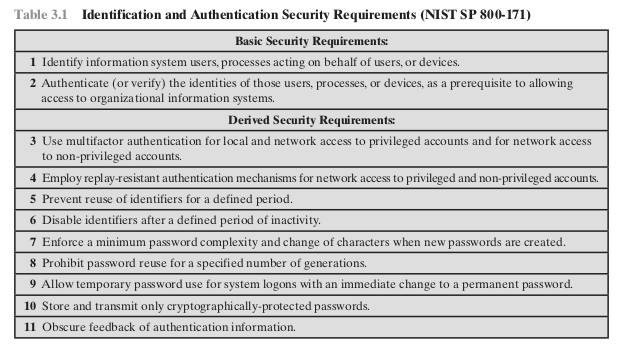
\includegraphics[width=14cm, keepaspectratio]{Bistarelli/img/cap_3/tabella3.1.png}
\end{figure}

\begin{figure}[H]
	\centering
    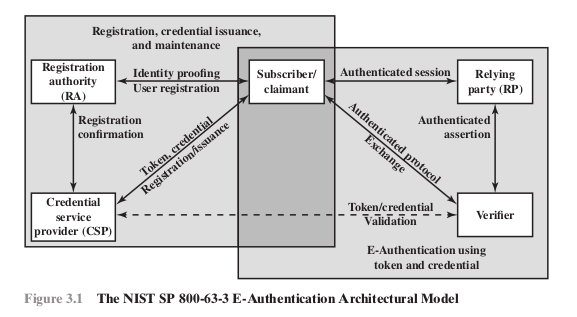
\includegraphics[width=14cm, keepaspectratio]{Bistarelli/img/cap_3/foto3.1.png}
\end{figure}


Una volta che un utente è registrato come abbonato, l'effettivo processo di autenticazione può avvenire tra l'abbonato e uno o più sistemi che eseguono l'autenticazione e, successivamente, l'autorizzazione. La parte che deve essere autenticata è chiamata richiedente e la parte che verifica tale identità è chiamata verificatore. Quando un richiedente dimostra con successo il possesso e il controllo di un token a un verificatore attraverso un protocollo di autenticazione, il verificatore può verificare che il richiedente sia il sottoscrittore indicato nella credenziale corrispondente. Il verificatore passa un'asserzione sull'identità del sottoscrittore alla parte fidata (RP).

\newpage
\subsection{Mezzi di Autenticazione}
Ci sono quattro mezzi generali per autenticare l'identità di un utente, che possono essere usati da soli o in combinazione:
\begin{enumerate}
    \item \textbf{Qualcosa che l'individuo conosce}
    
    Come una password, un numero di identificazione personale (PIN), o le risposte a una serie di domande prestabilite.
    
    \item \textbf{Qualcosa che l'individuo possiede}
    
    Come le keycard elettroniche, smart card e chiavi fisiche. Questo tipo di autenticatore è chiamato token.
    
    \item \textbf{Qualcosa che l'individuo è (biometria statica)}
    
    Come il riconoscimento per impronta digitale, retina e faccia.
    
    \item \textbf{Qualcosa che l'individuo fa (biometria dinamica)}
    
    Come il riconoscimento tramite il modello di voce, le caratteristiche della scrittura a mano e il ritmo di battitura.
\end{enumerate}
Tutti questi metodi, correttamente implementati e utilizzati, possono fornire un'autenticazione l'autenticazione dell'utente. Tuttavia, ogni metodo ha dei problemi. Un avversario può essere in grado di indovinare o rubare una password. Allo stesso modo, un avversario può essere in grado di falsificare o rubare un token. Un utente può dimenticare una password o perdere un token. 
\paragraph{L'autenticazione a più fattori} si riferisce all'uso di più di uno dei mezzi di autenticazione nella lista precedente. La forza dei sistemi di autenticazione è ampiamente determinata dal numero di fattori incorporati dal sistema. Le implementazioni che usano due fattori sono considerate più forti di quelle che usano un solo fattore. I sistemi che incorporano tre fattori sono più forti di quelli che ne incorporano solo due, e così via.

\newpage
\subsection{Valutazione dei rischi per l'autenticazione degli utenti}
Ci sono tre concetti separati che vogliamo mettere in relazione l'uno con l'altro: livello di sicurezza, impatto potenziale e aree di rischio.

\begin{itemize}
    \item \textbf{Livello di sicurezza}

Un livello di sicurezza descrive il grado di certezza di un'organizzazione che un utente ha presentato una credenziale che si riferisce alla sua identità. Più specificamente, la sicurezza è definita come:

    \item \textbf{Il grado di fiducia nel processo di controllo} utilizzato per stabilire l'identità dell'individuo a cui la credenziale è stata rilasciata.
    
    \item \textbf{Il grado di fiducia che l'individuo} che utilizza la credenziale sia l'individuo a cui la credenziale è stata rilasciata.
\end{itemize}
\paragraph{SP 800-63-3 riconosce quattro livelli di sicurezza:}
\begin{enumerate}
    \item \textbf{Livello:} poca o nessuna fiducia nella validità dell'identità asserita.
    
Un esempio in cui questo livello è appropriato è un consumatore che si registra per partecipare a una discussione sul sito web di un'azienda. La tipica tecnica di autenticazione a questo tipica a questo livello sarebbe un ID e una password forniti dall'utente al momento della transazione.
    
    \item \textbf{Livello:} una certa fiducia nella validità dell'identità asserita.

Le credenziali di livello 2 sono appropriate per un'ampia gamma di affari con il pubblico dove le organizzazioni che richiedono un'affermazione iniziale dell'identità (i cui dettagli sono verificati indipendentemente prima di qualsiasi azione). A questo livello, deve essere usato un qualche tipo di protocollo qualche tipo di protocollo di autenticazione sicura deve essere usato, insieme a uno dei mezzi di autenticazione riassunti in precedenza e discussi nelle sezioni successive.

    \item \textbf{Livello:} Alta fiducia nella validità dell'identità asserita
Questo livello è appropriato per permettere ai clienti o agli impiegati di accedere a servizi limitati di alto valore ma non al valore più alto.


    \item\textbf{Livello:} Fiducia molto alta nella validità dell'identità asserita
Questo livello è appropriato per permettere ai clienti o agli impiegati di accedere a servizi limitati di alto valore o per i quali un accesso improprio è molto dannoso.
\end{enumerate}

Un concetto strettamente legato a quello di livello di sicurezza è \textbf{il potenziale d'impatto}, definisce tre livelli di impatto potenziale sulle organizzazioni o sugli individui in caso di violazione della sicurezza (nel nostro contesto, un errore nell'autenticazione autenticazione dell'utente):

\begin{center}
    \textbf{Potenziale D'impatto}
\end{center}

\begin{itemize}
    \item \textbf{Low} Un errore di autenticazione potrebbe avere un effetto negativo limitato sulle operazioni organizzative, sulle risorse organizzative o sugli individui. Più specificamente, possiamo dire che l'errore potrebbe:
    
    \begin{itemize}
        \item Causare una degradazione della capacità capacità di missione in misura e durata tali che l'organizzazione sia in grado di eseguire le sue funzioni primarie, ma l'efficacia delle funzioni è notevolmente ridotta
        
        \item Provocare un danno minore ai beni dell'organizzazione
        
        \item Provocare una perdita finanziaria minore perdita finanziaria per l'organizzazione o gli individui
        
        \item Risultare in un danno minore agli individui.
    \end{itemize}
    
    \item \textbf{Moderate} Un errore di autenticazione potrebbe avere un serio effetto negativo effetto. Più specificamente, l'errore potrebbe:
    
    \begin{itemize}
        \item Causare una degradazione significativa nella capacità della missione in una misura e durata tale che l'organizzazione è in grado di eseguire le sue funzioni primarie, ma l'efficacia delle funzioni è significativamente.
        
        \item Provocare un danno significativo ai beni dell'organizzazione
        
        \item Provocare comporti una perdita finanziaria significativa
        
        \item Comporti un danno significativo alle persone che non che non implichi la perdita di vite umane o lesioni gravi in pericolo di vita.
    \end{itemize}
    \item \textbf{High}
    Un errore di autenticazione potrebbe avere un effetto negativo grave o catastrofico. L'errore potrebbe:
    \begin{itemize}
        \item Causare una grave degradazione o perdita della capacità della missione in misura e durata tali che l'organizzazione non sia in grado di eseguire una o più delle sue funzioni primarie
        
        \item Causare un grave danno ai beni dell'organizzazione
        
        \item Causare una grave perdita finanziaria all'organizzazione o agli individui
        
        \item Causare un danno grave o catastrofico agli individui che comporta la perdita della vita o lesioni gravi che mettono in pericolo la vita.
    \end{itemize}

\end{itemize}

La mappatura tra l'impatto potenziale e il livello appropriato di garanzia che è soddisfacente per affrontare l'impatto potenziale dipende dal contesto. La tabella 3.2 mostra una possibile mappatura per vari rischi a cui un'organizzazione può essere esposta. Questa tabella suggerisce una tecnica per fare la valutazione dei rischi. Per un dato sistema informativo o asset di servizio di un'organizzazione, l'organizzazione deve determinare il livello di impatto se si verifica un errore di autenticazione, usando le categorie di impatto, o aree di rischio, che sono preoccupanti. Per esempio, considerate il potenziale di perdita finanziaria se c'è un errore di autenticazione che risulta in un accesso non autorizzato a un database. A seconda della natura del del database, l'impatto potrebbe essere:

\begin{center}
    \textbf{Area di Rischio}
\end{center}

\begin{itemize}
    \item \textbf{Low} Nel peggiore dei casi, una perdita finanziaria insignificante o irrilevante perdita per qualsiasi parte, o nel peggiore dei casi, un'organizzazione insignificante o irrilevante responsabilità.
    
    \item \textbf{Moderate} Nel peggiore dei casi, una grave perdita finanziaria irrecuperabile per qualsiasi parte, o una grave responsabilità dell'organizzazione.

    
    \item \textbf{High} Grave o catastrofica perdita finanziaria irrecuperabile per qualsiasi parte; o grave o catastrofica responsabilità dell'organizzazione.
\end{itemize}
\newpage
\section{Autenticazione basata su password}

Una linea di difesa molto usata contro gli intrusi è il sistema di password. Praticamente tutti i sistemi multiutente, server basati sulla rete, siti di e-commerce basati sul web e altri servizi simili richiedono che un utente fornisca non solo un nome o un identificatore (ID) ma anche una password. Il sistema confronta la password con una password precedentemente memorizzata per quell'ID utente, conservata in un file di password di sistema. La password serve ad autenticare l'ID dell'individuo che accede al sistema. A sua volta, l'ID fornisce sicurezza nei seguenti modi:
\begin{itemize}
    \item \textbf{L'ID determina se l'utente è autorizzato ad accedere ad un sistema.}
    
    In alcuni sistemi, solo coloro che hanno già un ID depositato nel sistema sono permesso di accedere.
    
    \item \textbf{L'ID determina i privilegi accordati all'utente.}
    
    Alcuni utenti possono avere lo stato di amministratore o "superutente" che permette loro di leggere file ed eseguire funzioni che sono particolarmente protette dal sistema operativo. Alcuni sistemi hanno account ospiti o anonimi, e gli utenti di questi account hanno privilegi più privilegi più limitati degli altri.
    
    \item \textbf{L'ID è usato in quello che viene chiamato controllo di accesso discrezionale.}
    
    Per esempio esempio, elencando gli ID degli altri utenti, un utente può concedere loro il permesso di leggere i file di proprietà di quell'utente.
\end{itemize}
\newpage
\subsection{Vulnerabilità delle password}
\begin{itemize}
    \item \textbf{Attacco a dizionario offline:}
    
L'attaccante ottiene il file delle password di sistema e confronta gli hash delle password con gli hash delle password comunemente usate. Se viene trovata una corrispondenza, l'attaccante può ottenere l'accesso con quella combinazione ID/password.

        \begin{itemize}
            \item \textbf{Contromisure} 
            
            Includono controlli per prevenire l'accesso non autorizzato al file delle password, misure di rilevamento delle intrusioni per identificare una compromissione, e una rapida riemissione delle password se il file delle password viene compromesso.
        \end{itemize}

\item \textbf{Attacco all'account specifico}

L'attaccante prende di mira un account specifico e presenta password indovinate finché non viene scoperta la password corretta.

    \begin{itemize}
        \item \textbf{Contromisure} 
        
        è un meccanismo di blocco dell'account, che blocca l'accesso all'account dopo un certo numero di tentativi di accesso falliti. La pratica tipica è non più di di cinque tentativi di accesso.
    \end{itemize}

\item \textbf{Attacco con password popolare}

Una variante dell'attacco precedente consiste nell'utilizzare una password popolare e provarla contro una vasta gamma di ID utente. La tendenza di un utente è quella di scegliere una password che sia facilmente ricordabile; questo purtroppo rende la password facile da indovinare.

    \begin{itemize}
        \item \textbf{Contromisure} 
        
        Includono politiche per inibire la selezione da parte degli utenti di password comuni e la scansione degli indirizzi IP delle richieste di autenticazione e dei cookie del client per i modelli di invio.
    \end{itemize}

\item\textbf{Indovinare la password contro un singolo utente}

L'attaccante tenta di ottenere la conoscenza del titolare dell'account e delle politiche di password del sistema e usa tale conoscenza per indovinare la password.

    \begin{itemize}
        \item \textbf{Contromisure}
        
        Includono la formazione e l'applicazione di politiche sulle password che rendono le password difficili da indovinare.
    \end{itemize} 

\item\textbf{Dirottamento della stazione di lavoro}
L'attaccante aspetta fino a quando una stazione di lavoro loggata non è sorvegliata.

\begin{itemize}
    \item\textbf{Contromisure}
    
    è la registrazione automatica della workstation dopo un periodo di inattività. Gli schemi di rilevamento delle intrusioni possono essere usati per rilevare i cambiamenti nel comportamento dell'utente.
\end{itemize}

\item \textbf{Sfruttare gli errori dell'utente}

Se il sistema assegna una password, allora l'utente è più probabile che la scriva perché è difficile da ricordare. Questa situazione crea il potenziale per un avversario di leggere la password scritta. Un utente può condividere intenzionalmente una password, per permettere ad un collega di condividere i file, per esempio. Inoltre, gli aggressori hanno spesso successo nell'ottenere le password utilizzando tattiche di ingegneria sociale tattiche di ingegneria sociale che ingannano l'utente o un account manager a rivelare una password. Molti sistemi informatici sono forniti con password preconfigurate per gli amministratori di sistema. A meno che queste password preconfigurate non vengano cambiate, sono facilmente indovinate.

\begin{itemize}
    \item \textbf{Contromisure}
    
     la formazione degli utenti, il rilevamento delle intrusioni e password più semplici combinate con un altro meccanismo di autenticazione.
\end{itemize}

\item\textbf{Sfruttare l'uso di password multiple}

Gli attacchi possono anche diventare molto più efficaci o dannosi se diversi dispositivi di rete condividono la stessa password o una password simile per un dato utente. 

\begin{itemize}
    \item \textbf{Contromisure} 
    
    includono una politica che proibisce la stessa o password simili su particolari dispositivi di rete.
\end{itemize}
\newpage
\item \textbf{Monitoraggio elettronico}

Se una password viene comunicata attraverso una rete per accedere ad un sistema remoto, è vulnerabile alle intercettazioni. La semplice crittografia non risolve questo problema, perché la password criptata è, in effetti, la password e può essere osservata e riutilizzata da un avversario.
\end{itemize}
\subsection{Uso di password con hash}
Una tecnica di sicurezza delle password molto diffusa è l'uso di password con hash e di un valore di sale. Questo schema è presente in quasi tutte le varianti di UNIX e in numerosi altri sistemi operativi. Si utilizza la seguente procedura (vedi Figura 3.3). Per caricare una nuova password nel sistema, l'utente sceglie o gli viene assegnata una password. Questa password viene combinata con un valore di sale a lunghezza fissa. Nelle vecchie implementazioni, questo valore è legato al momento in cui la password è stata assegnata all'utente. 
\\
Le implementazioni più recenti utilizzano un numero pseudorandom o casuale. La password e il sale servono come input a un algoritmo di hashing per produrre un codice hash di lunghezza fissa.
\\
L'algoritmo di hash è progettato per essere lento nell'esecuzione al fine di contrastare gli attacchi. La password
hash viene memorizzata, insieme a una copia in chiaro del sale, nel file delle password dell'ID utente corrispondente.
file delle password per l'ID utente corrispondente. È stato dimostrato che il metodo della password hash è sicuro contro una serie di attacchi crittoanalitici.
\\
Quando un utente tenta di accedere a un sistema UNIX, fornisce un ID e una password (vedi Figura 3.1). e una password (vedi Figura 3.3b). Il sistema operativo utilizza l'ID per indicizzare il file delle password e recuperare "il sale" in chiaro e la password crittografata. "Il sale" e la password forniti dall'utente vengono utilizzati come input per la routine di crittografia. Se il risultato corrisponde al valore memorizzato, la password viene accettata.
\newpage
\paragraph{Il "sale" ha tre funzioni:}
\begin{enumerate}
    \item Impedisce che le password duplicate siano visibili nel file delle password. 
    
    Anche se due utenti scelgono la stessa password, a queste password saranno assegnati valori di valori di sale diversi. Di conseguenza, le password con hash dei due utenti saranno diverse.
    
    \item Questo aumenta notevolmente la difficoltà degli attacchi a dizionario offline. 
    
    Per un sale di lunghezza bits, il numero di password possibili aumenta di un fattore 2b, aumentando la difficoltà di indovinare una password la difficoltà di indovinare una password in un attacco a dizionario.
    
    \item Diventa quasi impossibile scoprire se una persona che ha password su due o più sistemi due o più sistemi abbia usato la stessa password su tutti.
    
\end{enumerate}

Per capire il secondo punto, considerate il modo in cui funzionerebbe un attacco a dizionario offline. L'attaccante ottiene una copia del file delle password. Supponiamo innanzitutto che il sale non venga utilizzato. L'obiettivo dell'attaccante è indovinare una singola password. A tal fine, l'attaccante sottopone alla funzione di hashing un gran numero di password probabili. Se una delle ipotesi corrisponde a uno degli hash del file, l'attaccante ha trovato una password che si trova nel file. Ma con lo schema UNIX, l'aggressore deve prendere ogni ipotesi e sottoporla alla funzione di hash una volta per ogni valore di sale nel file del dizionario, moltiplicando il numero di ipotesi da verificare. Lo schema di password UNIX è soggetto a due minacce. In primo luogo, un utente può ottenere l'accesso a una macchina utilizzando un account ospite o con altri mezzi e poi eseguire un programma per indovinare le password, chiamato password cracker, su quella macchina. L'attaccante dovrebbe essere in grado di controllare molte migliaia di possibili password con un consumo minimo di risorse. Inoltre, se l'avversario è in grado di ottenere una copia del file della password, il programma di cracking può essere eseguito a piacere su un altro computer. In questo modo, l'avversario può esaminare milioni di possibili password in un periodo di tempo ragionevole.

\begin{figure}[H]
	\centering
    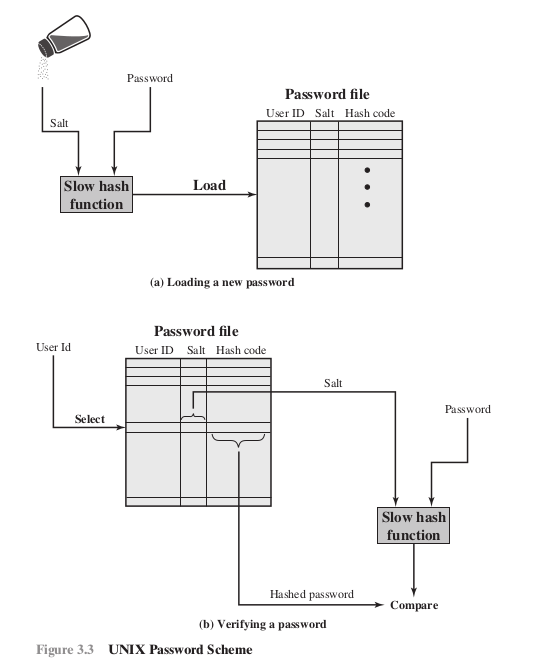
\includegraphics[width=14cm, keepaspectratio]{Bistarelli/img/cap_3/foto3.3.png}
\end{figure}
\newpage
\subsection{Cracking delle password scelte dall'utente}
\paragraph{Approccio Tradizionale}
L'approccio tradizionale all'indovinare le password, è quello di sviluppare un grande dizionario di possibili password e di provare ognuna di queste con il file delle password. Questo significa che ogni password deve essere sottoposta a un hash usando ogni valore di sale disponibile e poi confrontata con i valori di hash memorizzati. Se non viene trovata alcuna corrispondenza, il programma di cracking prova variazioni su tutte le parole del suo dizionario di password probabili. Tali variazioni includono l'ortografia a ritroso delle parole, numeri aggiuntivi o caratteri speciali, o sequenze di caratteri. Un'alternativa è quella di barattare lo spazio con il tempo precompilando i potenziali valori di hash. In questo approccio l'attaccante genera un grande dizionario di possibili password. Per ogni password, l'attaccante genera i valori di hash associati ad ogni possibile valore di sale. Il risultato è una mastodontica tabella di valori di hash nota come tabella arcobaleno.
\\
\paragraph{Approccio Moderno}
Purtroppo, questo tipo di vulnerabilità non è diminuita negli ultimi 25 anni o giù di lì. Gli utenti stanno facendo un lavoro migliore nel selezionare le password e le organizzazioni e le organizzazioni stanno facendo un lavoro migliore nel costringere gli utenti a scegliere password più forti, un concetto noto come politica delle password complesse. Tuttavia, le tecniche di cracking delle password sono migliorate per tenere il passo. I miglioramenti sono di due tipi. In primo luogo, la capacità di elaborazione disponibile per il cracking delle password è aumentata drammaticamente. Ora utilizzati sempre più per il calcolo, i processori grafici permettono ai programmi di cracking delle password di lavorare migliaia di volte più velocemente di quanto non facessero solo un dieci anni fa su PC di prezzo simile che usavano solo CPU tradizionali. Un PC che esegue una singola GPU AMD Radeon HD7970, per esempio, può provare in media una 8,2 * 109 combinazioni di password ogni secondo, a seconda dell'algoritmo utilizzato.
\singlespacing
La seconda area di miglioramento nel cracking delle password è l'uso di algoritmi sofisticati per generare potenziali password. I migliori risultati sono stati raggiunti studiando esempi di parole in uso. Per sviluppare tecniche che siano più efficienti ed efficaci dei semplici dizionario e degli attacchi brute-force, ricercatori e hacker hanno studiato la struttura struttura delle password. Per fare questo, gli analisti hanno bisogno di un grande pool di password di parole reali da studiare, cosa che ora hanno. La prima grande svolta è avvenuta alla fine del 2009, quando un attacco SQL injection contro il servizio di giochi online RockYou.com ha esposto 32 milioni di password in chiaro usate dai suoi membri per accedere ai loro account. Da da allora, numerosi set di file di password trapelate sono diventati disponibili per l'analisi.
\newpage
\subsection{Controllo dell'accesso ai file di password}
Un modo per contrastare un attacco con password è negare all'avversario l'accesso al file delle password. Se la porzione di password hash del file è accessibile solo da un utente privilegiato, allora l'avversario non può leggerla senza conoscere già la password di un utente privilegiato. Spesso, le password hash sono tenute in un file separato dagli ID utente, indicato come un file di password ombra.

Si presta particolare attenzione a rendere il file shadow password protetto da accessi non autorizzati. Anche se la protezione del file delle password sia certamente utile, rimangono delle vulnerabilità:

\begin{itemize}
    \item Molti sistemi, compresa la maggior parte dei sistemi UNIX, sono suscettibili di intrusioni.

Un hacker potrebbe essere in grado di sfruttare una vulnerabilità del software nel sistema operativo sistema operativo per bypassare il sistema di controllo degli accessi abbastanza a lungo da estrarre il file di password. In alternativa, l'hacker può trovare una debolezza nel file system o nel sistema di gestione del database che permette l'accesso al file.

    \item Un incidente di protezione potrebbe rendere il file delle password leggibile, rendendo così compromessi tutti gli account.

    \item Alcuni utenti hanno account su altre macchine in altri domini di protezione, e usano la stessa password. Quindi, se le password potrebbero essere lette da chiunque su una macchina, una macchina in un'altra posizione potrebbe essere compromessa.

    \item Una mancanza o una debolezza nella sicurezza fisica può fornire opportunità per un hacker.

A volte, c'è un backup del file delle password su un disco di riparazione disco di riparazione di emergenza o un disco di archiviazione. L'accesso a questo backup permette all'attaccante di leggere il file della password. In alternativa, un utente può avviare da un disco che esegue un altro sistema operativo come Linux e accedere al file da questo sistema operativo.


    \item Invece di catturare il file delle password di sistema, un altro approccio per raccogliere ID utente e password è attraverso lo sniffing del traffico di rete.
\end{itemize}
\singlespacing
Quindi, una politica di protezione delle password deve integrare le misure di controllo dell'accesso con tecniche per forzare gli utenti a scegliere password difficili da indovinare.
\newpage
\subsection{Strategie selezione password}
Quando non sono costretti, molti utenti scelgono una password troppo corta o troppo facile da indovinare. All'altro estremo, se agli utenti vengono assegnate password che consistono di otto caratteri stampabili scelti a caso, il cracking della password è effettivamente impossibile. Ma sarebbe quasi altrettanto impossibile per la maggior parte degli utenti ricordare le loro password. Il nostro obiettivo, quindi, è quello di eliminare le password indovinabili mentre permettendo all'utente di scegliere una password che sia memorizzabile. Quattro tecniche di base sono in uso:
\begin{enumerate}
    \item Educazione dell'utente
    \item Password generate dal computer
    \item Controllo reattivo delle password
    \item Politica delle password complesse
\end{enumerate}
\singlespacing
Gli utenti possono essere informati dell'importanza di usare password difficili da indovinare e possono essere fornire delle linee guida per la selezione di password forti. Questa strategia di educazione degli utenti è improbabile che abbia successo nella maggior parte delle installazioni, in particolare dove c'è una grande una vasta popolazione di utenti o molto turnover. Molti utenti semplicemente ignoreranno le linee guida. Altri possono non essere buoni giudici di ciò che è una password forte. Per esempio, molti utenti (erroneamente) credono che invertire una parola o scrivere in maiuscolo l'ultima lettera renda una password indovinabile
\newpage
\section{Autenticazione Basata sui token}
Gli oggetti che un utente possiede ai fini dell'autenticazione sono chiamati token.
\subsection{Memory Cards}
Le \textbf{Memory Cards} possono immagazzinare ma non elaborare dati.
\singlespacing
La più comune di queste carte è la carta bancaria con una banda magnetica sul retro. Una banda magnetica può memorizzare solo un semplice codice di sicurezza, che può essere letto (e sfortunatamente riprogrammato) da un economico lettore di carte. Ci sono anche schede di memoria che includono una memoria elettronica interna. Le carte di memoria possono essere usate da sole per
\begin{itemize}
    \item l'accesso fisico, come ad esempio in una stanza d'albergo.
    \item Per autenticazione, un utente fornisce sia la scheda di memoria che una qualche forma di password o numero di identificazione personale (PIN).
    
    Un'applicazione tipica è uno sportello automatico automatico (ATM). La scheda di memoria, se combinata con un PIN o una password, fornisce una sicurezza significativamente maggiore di una password da sola. Un avversario deve ottenere il possesso fisico possesso fisico della carta (o essere in grado di duplicarla) e in più deve ottenere la conoscenza del PIN. 
    \singlespacing
    Tra i potenziali inconvenienti NIST SP 800-12 (An Introduction to Computer Sicurezza: The NIST Handbook, ottobre 1995) nota quanto segue:
    \begin{itemize}
        \item \textbf{Richiede un lettore speciale}
        
        Questo aumenta il costo di utilizzo del token e crea l'obbligo di mantenere la sicurezza dell'hardware e del software del lettore.
        
        \item \textbf{Perdita dei token} 
        
        Un token perso impedisce temporaneamente al suo proprietario di ottenere l'accesso al sistema. Quindi, c'è un costo amministrativo nella sostituzione del token perso. Inoltre, se il token viene trovato, rubato o falsificato, allora un avversario deve solo determinare il PIN per ottenere un accesso non autorizzato.
        
        \item \textbf{Insoddisfazione dell'utente}
        
        Anche se gli utenti possono non avere difficoltà ad accettare l'uso di una scheda di memoria per l'accesso al bancomat, il suo uso per l'accesso al computer può essere considerato scomodo.
    \end{itemize}
\end{itemize}
\newpage
\subsection{Smart Cards}
Un'ampia varietà di dispositivi si qualificano come token intelligenti. Questi possono essere classificati lungo quattro dimensioni che non si escludono a vicenda:
\begin{itemize}
    \item \textbf{Caratteristiche fisiche} 
    
    I token intelligenti includono un microprocessore incorporato. Un token intelligente che assomiglia a una carta bancaria è chiamato smart card. Altri smart token possono assomigliare a calcolatrici, chiavi o altri piccoli oggetti portatili.
    
    \item \textbf{Interfaccia Utente}
    
    Le interfacce manuali includono una tastiera e un display per l'interazione uomo / interazione tra uomo e token.
     
    \item \textbf{Interfaccia Elettronica}
    
    Una smart card o un altro token richiede un'interfaccia elettronica elettronica per comunicare con un lettore/scrittore compatibile.
    
    \singlespacing
    
    Una carta può avere uno o entrambi i seguenti tipi di interfaccia:
    
    \begin{itemize}
        \item \textbf{Contatto}
        
        Una smart card a contatto deve essere inserita in un lettore di smart card con una connessione diretta a una piastra di contatto conduttiva sulla superficie della carta (tipicamente placcata in oro).
        
        La trasmissione di comandi, dati e stato della carta avviene attraverso questi punti di contatto fisico.

        \item \textbf{Senza Contatto}
        
        Una carta senza contatto richiede solo la vicinanza di un lettore.
        
        Sia il lettore che la carta hanno un'antenna, e i due comunicano utilizzando frequenze radio. La maggior parte delle carte senza contatto derivano anche l'energia per il chip interno da questo segnale elettromagnetico. La portata è tipicamente da un mezzo a tre pollici per le carte non alimentate a batteria, ideale per applicazioni come l'ingresso in un edificio e il pagamento che richiedono un'interfaccia della carta molto veloce.
        
        \item \textbf{Protocollo di autenticazione}
        
        Lo scopo di un token intelligente è quello di fornire un mezzo per l'autenticazione dell'utente.
        
        \newpage
        
        Possiamo classificare i protocolli di autenticazione usati con token intelligenti in tre categorie:
        
        \begin{enumerate}
            \item \textbf{Statico}
            
            Con un protocollo statico, l'utente si autentica con il token, poi il token autentica l'utente al computer. L'ultima metà di questo protocollo è simile al funzionamento di un token di memoria.
            
            \item \textbf{Generatore dinamico di password}
            
            In questo caso, il token genera una password unica password unica periodicamente (ad esempio, ogni minuto). Questa password viene poi inserita nel sistema informatico per l'autenticazione, sia manualmente dall'utente o elettronicamente tramite il token. Il token e il sistema informatico devono essere inizializzati e mantenuti sincronizzati in modo che il computer conosca la password che è corrente per questo token.
            
            \item \textbf{Sfida-risposta}
            
            In questo caso, il sistema informatico genera una sfida, come una stringa casuale di numeri. Il token intelligente genera una risposta basata sulla sfida. Per esempio, si potrebbe usare la crittografia a chiave pubblica e il token potrebbe criptare la stringa di sfida con la chiave privata del token.
        \end{enumerate}
    \end{itemize}
\end{itemize}
\newpage
\subsection{Elettronic Identity Cards}
Un'applicazione di crescente importanza è l'uso di una smart card come carta d'identità nazionale per i cittadini. Una carta d'identità elettronica nazionale (eID) può servire agli stessi scopi di altre carte d'identità nazionali, e carte simili come la patente di guida, per l'accesso ai servizi governativi e commerciali. Inoltre, una carta eID può fornire una prova di identità più forte ed essere usata in una più ampia varietà di applicazioni. In effetti, una carta eID è una smart card che è stata verificata dal governo nazionale come valida e autentica.
\singlespacing
L'identity cards conterrà:
\begin{itemize}
    \item Dati personali 
    
    Come nome, data di nascita e indirizzo
    
    \item Numero del documento
    
    Un identificatore alfanumerico di nove caratteri unico per ogni carta.

    \item Numero di accesso alla carta (CAN)
    
    Un numero decimale casuale di sei cifre stampato sulla faccia della carta.
    
    \item Zona a lettura ottica (MRZ)
    
     Tre righe di testo leggibile dall'uomo e dalla macchina sul retro della carta. Anche questo può essere usato come password.
\end{itemize}
Le funzioni dell'identiry cards sono:
\begin{itemize}
    \item \textbf{ePass}
    
    Questa funzione è riservata all'uso governativo e memorizza una rappresentazione digitale dell'identità del titolare della carta. Questa funzione è simile a, e può essere usata per, un passaporto elettronico. Anche altri servizi governativi possono usare ePass. La funzione ePass deve essere implementata sulla carta.
    
    \item \textbf{eID}
    
    Questa funzione è per uso generale in una varietà di applicazioni governative e commerciali. applicazioni commerciali. La funzione eID memorizza un record di identità a cui i servizi autorizzati possono accedere con il permesso del titolare della carta. I cittadini scelgono se vogliono attivare questa funzione.
    
    \item \textbf{eSign}
    
    Questa funzione opzionale memorizza una chiave privata e un certificato che verifica la chiave; è usata per generare una firma digitale. Un centro di fiducia del settore privato emette il certificato.
\end{itemize}
\section{Autenticazione Biometrica}
Un sistema di autenticazione biometrica tenta di autenticare un individuo sulla base di le sue caratteristiche fisiche uniche. Queste includono:
\begin{itemize}
    \item \textbf{Caratteristiche statiche}
    
    come le impronte digitali, la geometria della mano, le caratteristiche del viso e i modelli della retina e dell'iride
    
    \item \textbf{Caratteristiche dinamiche}
    
    come l'impronta vocale e la firma.
\end{itemize}
In sostanza, la biometria si basa sul riconoscimento dei modelli. Rispetto alle password e ai token, l'autenticazione è tecnicamente più complessa e costosa. Sebbene sia usata in un numero di applicazioni specifiche, la biometria deve ancora maturare come strumento standard per l'autenticazione degli utenti ai sistemi informatici.
\subsection{Caratteristiche fisiche utilizzate nelle applicazioni biometriche}
Un certo numero di diversi tipi di caratteristiche fisiche sono in uso o in fase di studio per l'autenticazione dell'utente. Le più comuni sono le seguenti:

\begin{itemize}
    \item \textbf{Caratteristiche facciali}
    
    Le caratteristiche facciali sono il mezzo più comune per l'identificazione da uomo a uomo; quindi è naturale considerarle per l'identificazione tramite computer. L'approccio più comune è quello di definire le caratteristiche basate sulla posizione relativa e la forma delle caratteristiche facciali chiave, come occhi, sopracciglia, naso, labbra e forma del mento.
    
    \item \textbf{Impronte digitali}
    
    Le impronte digitali sono state usate come mezzo di identificazione per secoli, e il processo è stato sistematizzato e automatizzato in particolare per l'applicazione della legge. Un'impronta digitale è il modello di creste e solchi sulla superficie del polpastrello. Si ritiene che le impronte digitali siano uniche in l'intera popolazione umana. In pratica, il riconoscimento automatico delle impronte digitali e sistema di corrispondenza estrae un certo numero di caratteristiche dall'impronta digitale per memorizzarle come surrogato numerico del modello completo dell'impronta digitale.
    
    \item \textbf{Geometria della mano}

    I sistemi di geometria della mano identificano le caratteristiche della mano, compresa la forma, la lunghezza e la larghezza delle dita.
    
    \item \textbf{Modello della retina}
    
    Il modello formato dalle vene sotto la superficie della retina è unico e quindi adatto all'identificazione. Un sistema biometrico retinico ottiene un'immagine digitale del modello retinico proiettando un fascio di luce visiva o infrarossa a bassa intensità nell'occhio.
    
    \item \textbf{Iride}
    
    Un'altra caratteristica fisica unica è la struttura dettagliata dell'iride.
    
    \item \textbf{Firma}
    
    Ogni individuo ha uno stile unico di scrittura e questo si riflette specialmente nella firma, che è tipicamente una sequenza scritta frequentemente. Tuttavia, più campioni di firma di un singolo individuo non saranno identici.
    
    \item \textbf{La voce}
    
    Mentre lo stile della firma di un individuo riflette non solo gli unici attributi fisici dello scrittore ma anche l'abitudine alla scrittura che si è sviluppata, i modelli di voce sono più strettamente legati alle caratteristiche fisiche e anatomiche del parlante. Ciononostante, c'è ancora una variazione da campione a campione nel tempo dallo stesso parlante, complicando il compito di riconoscimento biometrico.
\end{itemize}
\newpage
\subsection{Funzionamento di un sistema di autenticazione biometrica}
Ogni individuo che deve essere incluso nel database degli utenti autorizzati deve prima essere iscritto al sistema. Questo è analogo all'assegnazione di una password a un utente. Per un sistema biometrico, l'utente presenta al sistema un nome e, tipicamente, un qualche tipo di password o PIN. Allo stesso tempo, il sistema rileva alcune caratteristiche biometriche di questo utente (ad esempio, l'impronta digitale del dito indice destro). Il sistema digitalizza l'input e poi estrae un insieme di caratteristiche che possono essere memorizzate come un numero o un insieme di numeri che rappresentano questa caratteristica biometrica unica; questo insieme di numeri viene chiamato template dell'utente. L'utente è ora iscritto al sistema, che mantiene per l'utente un nome (ID), forse un PIN o una password, e il valore biometrico.
\singlespacing
A seconda dell'applicazione, l'autenticazione dell'utente su un sistema biometrico comporta la verifica o l'identificazione.
\begin{itemize}
    \item \textbf{Verifica}
    
    è analoga a quella di un utente che accede a un sistema usando una scheda di memoria o una smart card accoppiata a una password o a un PIN. Per la verifica biometrica, l'utente inserisce un PIN e utilizza anche un sensore biometrico. Il sistema estrae la caratteristica corrispondente e la confronta con il modello memorizzato per questo utente. Se c'è una corrispondenza, allora il sistema autentica questo utente.
    
    \item \textbf{Identificazione}
    
    l'individuo usa il sensore biometrico ma non presenta informazioni aggiuntive. Il sistema quindi confronta il modello presentato con l'insieme dei modelli memorizzati. Se c'è una corrispondenza, l'utente viene identificato. Altrimenti, l'utente viene rifiutato.
\end{itemize}

\begin{figure}[H]
	\centering
    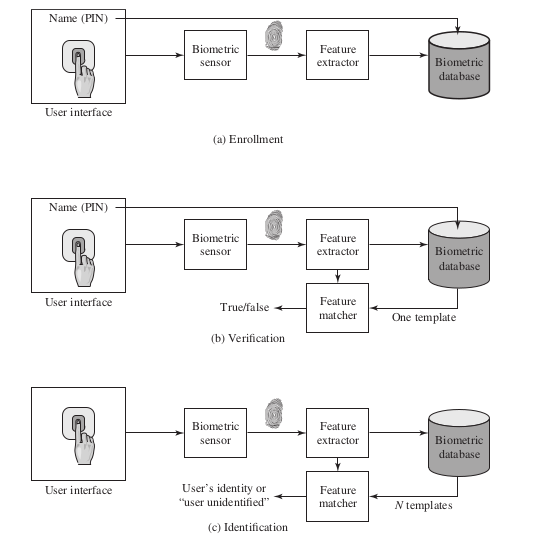
\includegraphics[width=14cm, keepaspectratio]{Bistarelli/img/cap_3/figura3.9.png}
\end{figure}

\begin{figure}[H]
	\centering
    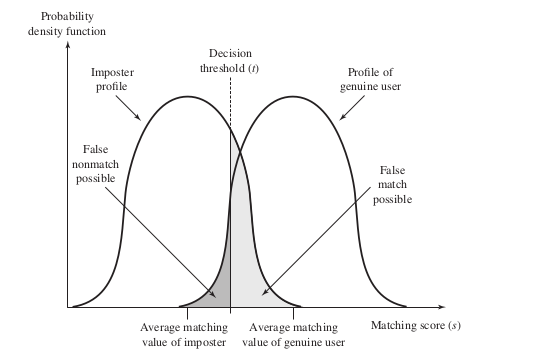
\includegraphics[width=14cm, keepaspectratio]{Bistarelli/img/cap_3/figura3.10.png}
\end{figure}
\subsection{Precisione Biometrica}
In qualsiasi schema biometrico, alcune caratteristiche fisiche dell'individuo sono mappate in una rappresentazione digitale. Per ogni individuo, una singola rappresentazione digitale, o template, è memorizzata nel computer. Quando l'utente deve essere autenticato, il sistema confronta il modello memorizzato con il modello presentato. Data la complessità delle caratteristiche fisiche, non ci si può aspettare che ci sia una corrispondenza esatta tra i due modelli. Piuttosto, il sistema usa un algoritmo per generare un punteggio (tipicamente un singolo numero) che quantifica la somiglianza tra l'input e il modello memorizzato. Per procedere con la discussione, definiamo i seguenti termini.
\begin{itemize}
    \item Il tasso di falsa corrispondenza
    
    è la frequenza con cui i campioni biometrici provenienti da diverse fonti diverse sono erroneamente valutati come provenienti dalla stessa fonte. Il tasso di falsa non corrispondenza è la frequenza con cui i campioni della stessa fonte sono erroneamente valutati essere di fonti diverse.
    
    \item La funzione di densità
    
    tipicamente forma una curva a campana.
\end{itemize}
\begin{figure}[H]
	\centering
    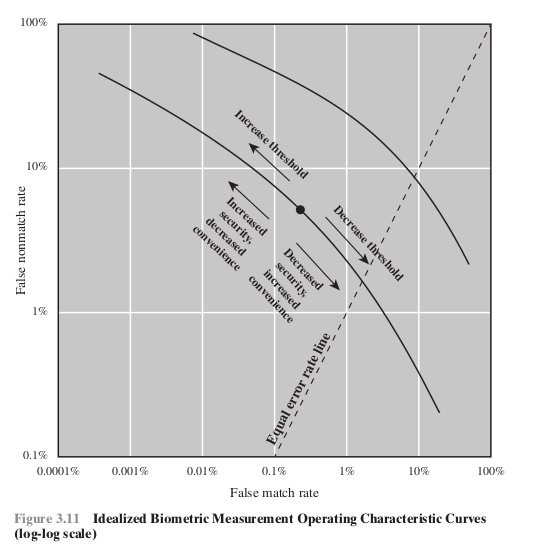
\includegraphics[width=14cm, keepaspectratio]{Bistarelli/img/cap_3/figura3.11.png}
\end{figure}
\singlespacing
\paragraph{Esempio} nel caso di un'impronta digitale, i risultati possono variare a causa del rumore del sensore, dei cambiamenti nell'impronta dovuti al gonfiore o alla secchezza, del posizionamento del dito e così via. In media, qualsiasi altro individuo dovrebbe avere un punteggio di corrispondenza molto più basso, ma ancora una volta mostrerà una funzione di densità di probabilità a campana. La difficoltà è che la gamma di punteggi di corrispondenza prodotti da due individui, uno autentico e uno impostore, rispetto a un dato modello di riferimento, è probabile che si sovrappongano. Nella figura 3.10, un valore di soglia è selezionato in modo che se il valore presentato s >= t si assume una corrispondenza, e per s < t, si assume una mancata corrispondenza. La parte ombreggiata a destra di t indica una gamma di valori per cui è possibile una falsa corrispondenza, e la parte ombreggiata a sinistra indica una gamma di valori per cui è possibile una falsa non corrispondenza. Una falsa corrispondenza comporta l'accettazione di un utente che non dovrebbe essere accettato, e una falsa mancata corrispondenza provoca il rifiuto di un utente valido. L'area di ogni parte ombreggiata rappresenta la probabilità di una falsa corrispondenza o non corrispondenza, rispettivamente. Spostando la soglia, a sinistra o a destra, le probabilità possono essere alterate, ma si noti che una diminuzione del tasso di falsi riscontri si traduce in un aumento del tasso di falsi non riscontri, e viceversa.
\section{Autenticazione Remota dell'utente}
La forma più semplice di autenticazione dell'utente è l'autenticazione locale, in cui un utente tenta di accedere a un sistema che è presente localmente, come un PC da ufficio stand-alone o un bancomat. Il caso più complesso è quello dell'autenticazione remota dell'utente, che avviene su Internet, una rete o un collegamento di comunicazione. L'autenticazione remota dell'utente solleva ulteriori minacce alla sicurezza, come un intercettatore in grado di catturare una password, o un avversario che riproduce una sequenza di autenticazione che è stata osservata.
\newpage
\subsection{Protocollo delle password}
In questo esempio, un utente trasmette prima la sua identità a all'host remoto. L'host genera un numero casuale r, spesso chiamato nonce, restituisce questo nonce all'utente.
\singlespacing
Inoltre, l'host specifica due funzioni, h() e f(), da utilizzare nella risposta. Questa trasmissione dall'host all'utente è la sfida. La risposta dell'utente è la quantità f(r', h(P')), dove r' = r e P' è la password dell'utente.
\singlespacing
La funzione h è una funzione hash, quindi la risposta consiste nella funzione hash della password dell'utente combinata con il numero casuale utilizzando la funzione.
\singlespacing
L'host memorizza la funzione hash della password di ogni utente registrato, rappresentata come h(P(U)) per l'utente U. Quando arriva la risposta, l'host confronta f(r', h(P')) con la f(r, h(P(U)) calcolata.) Se le quantità corrispondono, l'utente è autenticato. Questo schema difende da diverse forme di attacco. L'host memorizza non la password ma un codice hash della password. Questo protegge la password dagli intrusi nel sistema host. Inoltre, nemmeno l'hash della password viene trasmesso direttamente, ma piuttosto una funzione in cui l'hash della password è uno degli argomenti. Così, per una funzione f adatta, l'hash della password non può essere catturato durante la trasmissione.
\singlespacing
Infine, l'uso di un numero casuale tenta di difendere da un attacco di replay, in cui un avversario cattura la trasmissione dell'utente e tenta di accedere a un sistema ritrasmettendo i messaggi.
\begin{figure}[H]
	\centering
    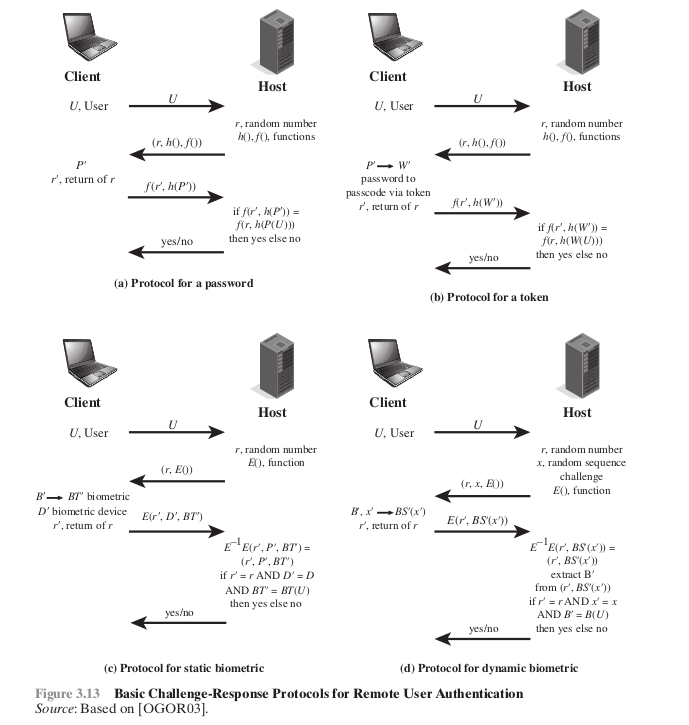
\includegraphics[width=14cm, keepaspectratio]{Bistarelli/img/cap_3/figura3.13.png}
\end{figure}
\subsection{Protocollo di Token}
Come prima, un utente trasmette prima la sua identità all'host remoto. L'host restituisce un numero casuale e gli identificatori delle funzioni f() e h() da utilizzare nella risposta. Alla fine dell'utente, il token fornisce un codice di accesso W'. Il token memorizza un codice statico statico o genera un codice casuale una tantum. Per un codice casuale una tantum, il token deve essere sincronizzato. Per un codice casuale una tantum, il token deve essere sincronizzato in qualche modo con l'host. In entrambi i casi, l'utente attiva il codice inserendo una password P'. Questa password è condivisa solo tra l'utente e il token e non coinvolge l'host remoto. Il token risponde all'host con la quantità f(r', h(W')). Per un codice di accesso statico, l host memorizza il valore hashed h(W(U)); per un passcode dinamico, l'host genera un passcode una tantum (sincronizzato con quello generato dal token) e prende il suo hash. L'autenticazione procede poi nello stesso modo del protocollo della password.
\subsection{Protocollo biometrico statico}
Come prima cosa, l'utente trasmette un ID all'host, che risponde con un numero casuale r e, in questo caso, l'identificatore di una crittografia E(). Sul lato utente c'è un sistema client che controlla un dispositivo biometrico. Il sistema genera un template biometrico BT' dal biometrico dell'utente B' e restituisce il testo cifrato E(r', D', BT'), dove D' identifica questo particolare dispositivo biometrico. L'host decifra il messaggio in arrivo per recuperare i tre parametri trasmessi e li confronta con i valori memorizzati localmente.
\singlespacing
Per una corrispondenza, l'host deve trovare r' = r. Inoltre, il punteggio di corrispondenza tra BT' e il modello memorizzato deve superare una soglia predefinita. Infine, l'host fornisce una semplice autenticazione del dispositivo di cattura biometrica confrontando l'ID del dispositivo in entrata con un elenco di dispositivi registrati nel database dell'host.
\subsection{Protocollo Biometrico Dinamico}
La principale differenza rispetto al caso di una biometria stabile è che l'host fornisce una sequenza casuale fornisce una sequenza casuale e un numero casuale come sfida. La sfida è una sequenza di numeri, caratteri o parole. L'utente umano all'estremità del client deve quindi vocalizzare (verifica con altoparlante), digitare (verifica dinamica della tastiera) o scrivere (verifica a mano) o scrivere (verifica della scrittura) la sequenza per generare un segnale biometrico BS'(x'). Il lato client cripta il segnale biometrico e il numero casuale. All'indirizzo lato host, il messaggio in arrivo viene decifrato. Il numero casuale in arrivo r' deve essere una corrispondenza esatta con il numero casuale che è stato originariamente utilizzato come sfida (r). Inoltre, l'host genera un confronto basato sul segnale biometrico in entrata biometrico BS'(x'), il template memorizzato BT(U) per questo utente e il segnale originale x. Se il valore di confronto supera una soglia predefinita, l'utente viene autenticato.